\appendix

\section{Per-Dataset Results of the Main Benchmark}
\label{app:perdataset}

Tables~\ref{tab:perdataset_classification} and~\ref{tab:perdataset_regression} give the primary metric for every model
and dataset (mean over 10 folds). All per-fold results, including the secondary metrics and timings, are in the
supplementary material.

\begin{table}[h]
\centering
\scriptsize
\setlength{\tabcolsep}{3pt}
\caption{Per-dataset log loss (classification), mean over 10 folds. Best value per dataset in bold.}
\label{tab:perdataset_classification}
\smallskip
\begin{adjustbox}{max width=\textwidth}
\begin{tabular}{lrrrrrrrr}
\toprule
Dataset & Kumo Tabular & Logistic reg. & Random forest & Extra trees & HistGB & XGBoost & LightGBM & CatBoost \\
\midrule
balance-scale & \textbf{0.024} & 0.278 & 0.535 & 2.853 & 0.407 & 0.319 & 0.331 & 0.255 \\
banknote-authentication & \textbf{0.000} & 0.048 & 0.027 & 0.014 & 0.015 & 0.015 & 0.023 & 0.008 \\
blood-transfusion-service-center & \textbf{0.468} & 0.477 & 0.782 & 2.490 & 0.579 & 0.609 & 0.559 & 0.490 \\
climate-model-simulation-crashes & 0.131 & \textbf{0.131} & 0.190 & 0.183 & 0.182 & 0.149 & 0.198 & 0.140 \\
diabetes & \textbf{0.466} & 0.485 & 0.480 & 0.483 & 0.632 & 0.721 & 0.628 & 0.480 \\
kc2 & \textbf{0.374} & 0.386 & 0.754 & 0.821 & 0.515 & 0.531 & 0.526 & 0.384 \\
mfeat-morphological & \textbf{0.559} & 0.643 & 0.944 & 4.116 & 1.143 & 0.887 & 1.126 & 0.648 \\
mfeat-zernike & \textbf{0.213} & 0.374 & 0.687 & 3.743 & 0.967 & 0.724 & 0.938 & 0.541 \\
pc1 & \textbf{0.160} & 0.227 & 0.181 & 0.545 & 0.297 & 0.240 & 0.315 & 0.180 \\
pc3 & \textbf{0.236} & 0.283 & 0.265 & 0.332 & 0.357 & 0.353 & 0.355 & 0.258 \\
pc4 & \textbf{0.157} & 0.229 & 0.197 & 0.224 & 0.236 & 0.223 & 0.226 & 0.180 \\
qsar-biodeg & \textbf{0.284} & 0.334 & 0.341 & 0.368 & 0.381 & 0.376 & 0.409 & 0.305 \\
steel-plates-fault & \textbf{0.383} & 0.773 & 0.577 & 0.573 & 0.669 & 0.568 & 0.647 & 0.506 \\
vehicle & \textbf{0.199} & 0.472 & 0.498 & 0.517 & 0.697 & 0.579 & 0.613 & 0.475 \\
wdbc & \textbf{0.062} & 0.078 & 0.112 & 0.108 & 0.110 & 0.091 & 0.119 & 0.082 \\
\bottomrule
\end{tabular}
\end{adjustbox}
\end{table}


\begin{table}[h]
\centering
\scriptsize
\setlength{\tabcolsep}{3pt}
\caption{Per-dataset RMSE (regression), mean over 10 folds. Best value per dataset in bold.}
\label{tab:perdataset_regression}
\smallskip
\begin{adjustbox}{max width=\textwidth}
\begin{tabular}{lrrrrrrrr}
\toprule
Dataset & Kumo Tabular & Linear reg. & Random forest & Extra trees & HistGB & XGBoost & LightGBM & CatBoost \\
\midrule
QSAR\_fish\_toxicity & \textbf{0.841} & 0.954 & 0.884 & 0.882 & 0.897 & 0.944 & 0.899 & 0.857 \\
airfoil\_self\_noise & \textbf{0.780} & 4.823 & 1.648 & 1.390 & 1.789 & 1.462 & 1.790 & 1.466 \\
cars & \textbf{2037.702} & 2944.899 & 2307.586 & 2418.453 & 2481.138 & 2389.355 & 2484.833 & 2111.137 \\
concrete\_compressive\_strength & \textbf{3.490} & 10.436 & 4.777 & 4.509 & 4.376 & 4.148 & 4.406 & 3.928 \\
energy\_efficiency & 0.416 & 2.943 & 0.449 & 0.438 & 0.482 & \textbf{0.289} & 0.482 & 0.291 \\
red\_wine & 0.570 & 0.651 & 0.559 & \textbf{0.543} & 0.586 & 0.595 & 0.587 & 0.573 \\
\bottomrule
\end{tabular}
\end{adjustbox}
\end{table}


\section{Case Studies: Breast Cancer and Diabetes}
\label{app:case}

The case studies use five stratified (classification) or random (regression) 80/20 splits with seeds 42--46, logistic
or linear regression, random forests (500 trees) and histogram gradient boosting with defaults, and Kumo Tabular with
the same settings as the main benchmark. Malignant tumours are the positive class. Tables~\ref{tab:classification}
and~\ref{tab:regression} report means and standard deviations over the splits; Table~\ref{tab:paired} the
within-dataset paired comparison with the strongest baseline; Tables~\ref{tab:study_classification}
and~\ref{tab:study_regression} the training-size study (seeds 42--44); and Figure~\ref{fig:case} the training-size
curves and Kumo Tabular's quantile intervals. Because five resampled splits are dependent, these analyses are
descriptive; no within-dataset difference is significant after the overlap correction and Holm's adjustment. A
complete re-run of the same code reproduced all metrics exactly, and execution of the same notebooks in a separate
cloud environment (NVIDIA T4, PyTorch 2.11,
float16) reproduced the results of Kumo Tabular, logistic/linear regression and random forests at the reported
precision; histogram gradient boosting differed slightly there (for example, accuracy 0.960 instead of 0.967).

\begin{table*}[t]
\centering
\caption{Breast cancer classification results (mean $\pm$ standard deviation over five stratified splits, 114 test rows each). Malignant is the positive class. Time is fit plus prediction time per split. Best mean per metric in bold.}
\label{tab:classification}
\setlength{\tabcolsep}{5pt}
\smallskip
\begin{adjustbox}{max width=\textwidth}
\begin{tabular}{lcccccc}
\toprule
Model & Accuracy & Precision & Recall & F1 & ROC-AUC & Time (s) \\
\midrule
Kumo Tabular & \textbf{0.989 $\pm$ 0.010} & \textbf{0.995 $\pm$ 0.010} & \textbf{0.976 $\pm$ 0.029} & \textbf{0.985 $\pm$ 0.014} & \textbf{0.998 $\pm$ 0.003} & 1.099 $\pm$ 0.012 \\
Logistic Reg. & 0.977 $\pm$ 0.012 & 0.990 $\pm$ 0.013 & 0.948 $\pm$ 0.031 & 0.968 $\pm$ 0.017 & 0.995 $\pm$ 0.004 & 0.019 $\pm$ 0.001 \\
Random Forest & 0.954 $\pm$ 0.013 & 0.947 $\pm$ 0.031 & 0.929 $\pm$ 0.024 & 0.938 $\pm$ 0.018 & 0.988 $\pm$ 0.011 & 1.204 $\pm$ 0.063 \\
HistGB & 0.967 $\pm$ 0.016 & 0.976 $\pm$ 0.024 & 0.933 $\pm$ 0.043 & 0.953 $\pm$ 0.022 & 0.994 $\pm$ 0.007 & 0.274 $\pm$ 0.020 \\
\bottomrule
\end{tabular}
\end{adjustbox}
\end{table*}


\begin{table*}[t]
\centering
\caption{Diabetes regression results (mean $\pm$ standard deviation over five random splits, 89 test rows each). Kumo Tabular uses the median quantile $q_{0.5}$ as point prediction. Best mean per metric in bold.}
\label{tab:regression}
\setlength{\tabcolsep}{5pt}
\smallskip
\begin{adjustbox}{max width=\textwidth}
\begin{tabular}{lcccc}
\toprule
Model & MAE & RMSE & $R^2$ & Time (s) \\
\midrule
Kumo Tabular & \textbf{42.48 $\pm$ 3.10} & \textbf{52.88 $\pm$ 3.47} & \textbf{0.503 $\pm$ 0.039} & 0.627 $\pm$ 0.053 \\
Linear Reg. & 43.75 $\pm$ 3.59 & 53.27 $\pm$ 4.03 & 0.496 $\pm$ 0.046 & 0.003 $\pm$ 0.000 \\
Random Forest & 45.23 $\pm$ 2.63 & 56.16 $\pm$ 3.31 & 0.440 $\pm$ 0.022 & 0.833 $\pm$ 0.024 \\
HistGB & 45.85 $\pm$ 0.72 & 58.52 $\pm$ 1.67 & 0.390 $\pm$ 0.042 & 0.190 $\pm$ 0.031 \\
\bottomrule
\end{tabular}
\end{adjustbox}
\end{table*}


\begin{table*}[t]
\centering
\caption{Paired comparison of Kumo Tabular with the strongest baseline over the five splits. $\overline{d}$ is the mean advantage of Kumo (positive favours Kumo for every metric), $s_d$ its standard deviation. The corrected test and interval use the Nadeau--Bengio variance correction for overlapping training sets; Holm adjustment is applied within each task. No result is significant at $\alpha=0.05$ after adjustment.}
\label{tab:paired}
\setlength{\tabcolsep}{4.5pt}
\smallskip
\begin{adjustbox}{max width=\textwidth}
\begin{tabular}{llcccccccc}
\toprule
Task & Metric & W/T/L & $\overline{d}$ & $s_d$ & Corrected 95\% CI & $p_{\mathrm{naive}}$ & $p_{\mathrm{corr}}$ & $p_{\mathrm{corr}}^{\mathrm{Holm}}$ & $p_{\mathrm{Wilcoxon}}$ \\
\midrule
Classification & Accuracy & 5/0/0 & 0.0123 & 0.0078 & [$-$0.0023, 0.0269] & 0.025 & 0.080 & 0.313 & 0.062 ($n$=5) \\
 & Precision & 2/3/0 & 0.0051 & 0.0111 & [$-$0.0156, 0.0258] & 0.362 & 0.531 & 0.535 & 0.500 ($n$=2) \\
 & Recall & 5/0/0 & 0.0286 & 0.0106 & [0.0087, 0.0484] & 0.004 & 0.016 & 0.081 & 0.062 ($n$=5) \\
 & F1 & 5/0/0 & 0.0172 & 0.0109 & [$-$0.0031, 0.0376] & 0.024 & 0.078 & 0.313 & 0.062 ($n$=5) \\
 & ROC-AUC & 4/1/0 & 0.0030 & 0.0034 & [$-$0.0034, 0.0094] & 0.126 & 0.267 & 0.535 & 0.125 ($n$=4) \\
\midrule
Regression & MAE & 4/0/1 & 1.27 & 1.10 & [$-$0.78, 3.32] & 0.061 & 0.161 & 0.484 & 0.125 ($n$=5) \\
 & RMSE & 3/0/2 & 0.39 & 1.43 & [$-$2.28, 3.07] & 0.573 & 0.704 & 1.000 & 0.625 ($n$=5) \\
 & $R^2$ & 3/0/2 & 0.007 & 0.028 & [$-$0.046, 0.060] & 0.603 & 0.727 & 1.000 & 0.625 ($n$=5) \\
\bottomrule
\end{tabular}
\end{adjustbox}
\end{table*}


\begin{table}[t]
\centering
\caption{Classification accuracy by training-set size (mean $\pm$ standard deviation over three seeds; full test split).}
\label{tab:study_classification}
\setlength{\tabcolsep}{3pt}
\begin{tabular}{rcccc}
\toprule
$n$ & Kumo Tabular & Logistic Reg. & Random Forest & HistGB \\
\midrule
25 & 0.950\,{\scriptsize$\pm$0.027} & \textbf{0.956}\,{\scriptsize$\pm$0.023} & 0.930\,{\scriptsize$\pm$0.018} & 0.632\,{\scriptsize$\pm$0.000} \\
50 & \textbf{0.953}\,{\scriptsize$\pm$0.051} & \textbf{0.953}\,{\scriptsize$\pm$0.022} & 0.933\,{\scriptsize$\pm$0.044} & 0.909\,{\scriptsize$\pm$0.035} \\
100 & \textbf{0.956}\,{\scriptsize$\pm$0.040} & \textbf{0.956}\,{\scriptsize$\pm$0.026} & 0.939\,{\scriptsize$\pm$0.015} & 0.944\,{\scriptsize$\pm$0.051} \\
200 & \textbf{0.985}\,{\scriptsize$\pm$0.013} & 0.971\,{\scriptsize$\pm$0.013} & 0.947\,{\scriptsize$\pm$0.009} & 0.947\,{\scriptsize$\pm$0.009} \\
400 & \textbf{0.982}\,{\scriptsize$\pm$0.015} & 0.974\,{\scriptsize$\pm$0.015} & 0.953\,{\scriptsize$\pm$0.018} & 0.956\,{\scriptsize$\pm$0.009} \\
455 & \textbf{0.988}\,{\scriptsize$\pm$0.013} & 0.974\,{\scriptsize$\pm$0.015} & 0.959\,{\scriptsize$\pm$0.013} & 0.959\,{\scriptsize$\pm$0.010} \\
\bottomrule
\end{tabular}
\end{table}


\begin{table}[t]
\centering
\caption{Regression $R^2$ by training-set size (mean $\pm$ standard deviation over three seeds; full test split).}
\label{tab:study_regression}
\setlength{\tabcolsep}{3pt}
\begin{tabular}{rcccc}
\toprule
$n$ & Kumo Tabular & Linear Reg. & Random Forest & HistGB \\
\midrule
25 & \textbf{0.429}\,{\scriptsize$\pm$0.058} & 0.075\,{\scriptsize$\pm$0.304} & 0.388\,{\scriptsize$\pm$0.127} & $-$0.097\,{\scriptsize$\pm$0.087} \\
50 & \textbf{0.437}\,{\scriptsize$\pm$0.019} & 0.331\,{\scriptsize$\pm$0.137} & 0.418\,{\scriptsize$\pm$0.008} & 0.348\,{\scriptsize$\pm$0.063} \\
100 & \textbf{0.486}\,{\scriptsize$\pm$0.045} & 0.467\,{\scriptsize$\pm$0.076} & 0.433\,{\scriptsize$\pm$0.024} & 0.410\,{\scriptsize$\pm$0.043} \\
200 & 0.505\,{\scriptsize$\pm$0.085} & \textbf{0.506}\,{\scriptsize$\pm$0.060} & 0.438\,{\scriptsize$\pm$0.057} & 0.391\,{\scriptsize$\pm$0.069} \\
353 & \textbf{0.526}\,{\scriptsize$\pm$0.028} & 0.507\,{\scriptsize$\pm$0.048} & 0.440\,{\scriptsize$\pm$0.024} & 0.406\,{\scriptsize$\pm$0.030} \\
\bottomrule
\end{tabular}
\end{table}


\begin{figure}[h]
\centering
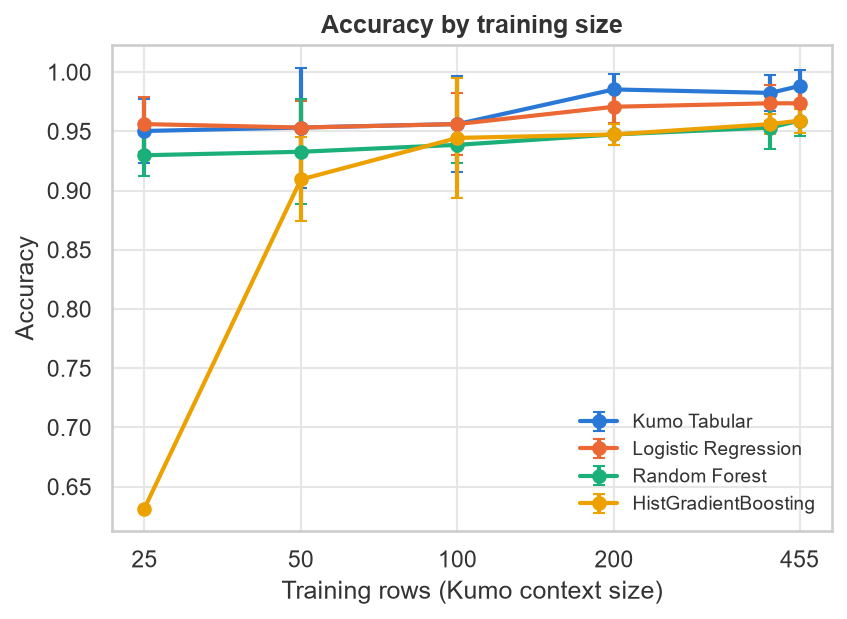
\includegraphics[width=0.32\textwidth]{figures/original_classification_sample_size_accuracy.png}\hfill
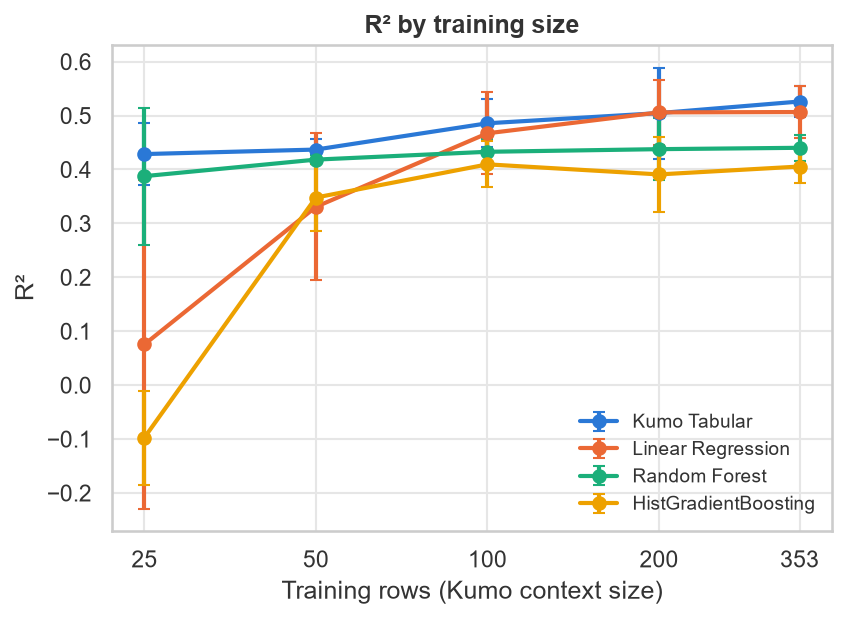
\includegraphics[width=0.32\textwidth]{figures/original_regression_sample_size_r2.png}\hfill
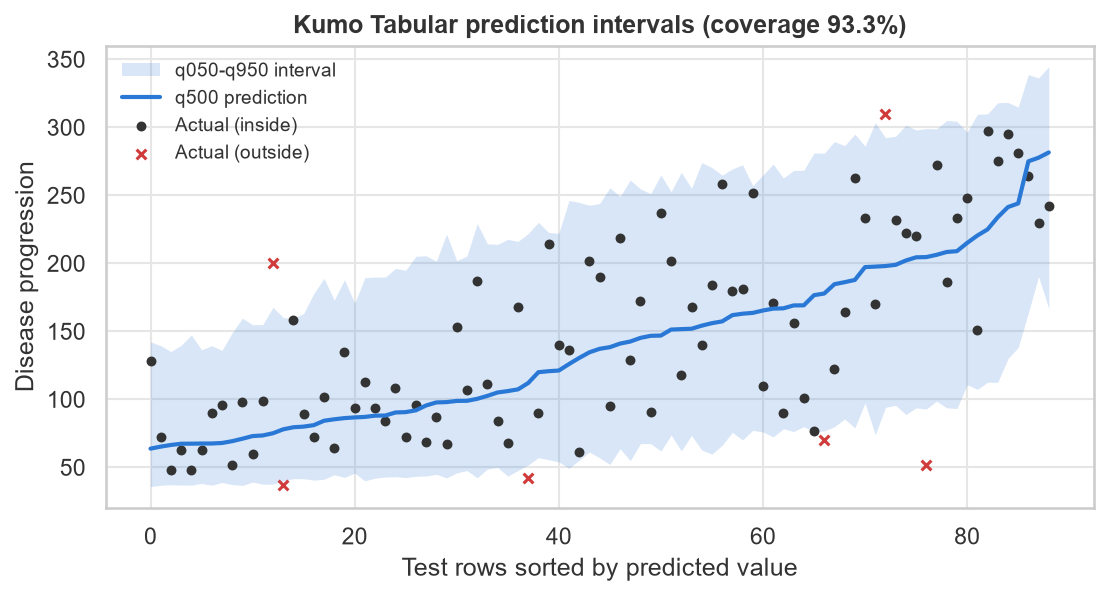
\includegraphics[width=0.32\textwidth]{figures/original_regression_kumo_intervals.png}
\caption{Case studies: classification accuracy and regression $R^2$ by number of training rows (mean $\pm$ one standard
deviation over three seeds; logarithmic horizontal axis), and Kumo Tabular's median prediction with its nominal 90\%
interval on one diabetes split (coverage 93.3\% on that split).}
\label{fig:case}
\end{figure}

\section{Software and Hardware}
\label{app:software}

Python 3.12.16, PyTorch 2.14.1 \citep{paszke2019pytorch} (CUDA 12.6), structured-data-models 0.2.1, scikit-learn 1.9.1, XGBoost 3.4.1, LightGBM
4.7.0, CatBoost 1.2.10, NumPy 2.5.4, pandas 3.1.0; NVIDIA GeForce GTX 980M (8\,GB, compute capability 5.2), Intel Core
i7-6700HQ, 16\,GB RAM, Windows 10. Kumo Tabular weights: Hugging Face repository \texttt{nvidia/Kumo-Tabular}, revision
\texttt{v1.0.1}, \texttt{small} checkpoints.
